\chapter{Controlador de corriente} \chapterlabel{Informe/4-ControladorCorriente} \label{cap:ControladorCorriente}
\section{Diseño y modelado}

\noindent Para regular la fuerza ejercida por el electroimán es necesario controlar la corriente que circula por él. Para ello, se modela a la planta como la impedancia de un inductor con una resistencia serie, cuya inductancia varía con el gap de aire:

\begin{equation} \label{eq1}
\frac{1}{sL(y)\ +\ R_L}
\end{equation}

\noindent Para realizar este control se utiliza un sistema realimentado, como el que se muestra en la figura \ref{fig:img_diag-en-bloques}. Se puede ver que se ingresa con una tensión de referencia ($V_{in}$) proporcional a la corriente de salida deseada, que luego se multiplica por la ganancia de entrada ($K_{in}$). La corriente del electroimán se realimenta en forma de una tensión proporcional a ella ($V_{iF}$). Ambas tensiones son restadas y el resultado (e) ingresa al bloque de comparador con histéresis, que actúa en conmutación, por lo que su salida tiene dos estados posibles: $\pm$$V_L$.

\noindent Al ser aplicadas al inductor se producirá una rampa de corriente: si la tensión es positiva, la rampa crece, y si es negativa decrece. De esta forma, debido a la conmutación del comparador se obtiene, a la salida, una forma de onda triangular $I_L$, cuyo valor medio es la corriente deseada y se corresponde a la tensión de referencia.

\begin{figure}[H]
	\centering
	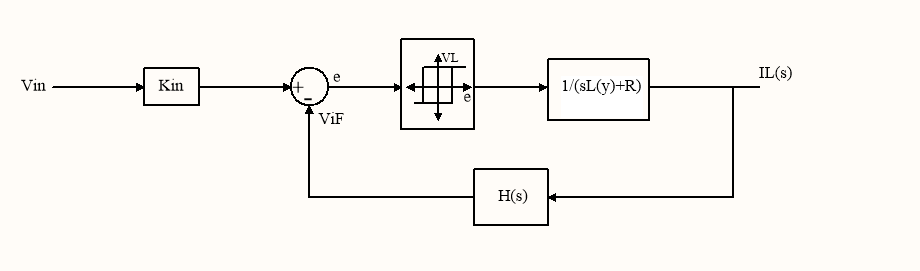
\includegraphics[width=\textwidth]{Diagrama-en-bloques.png}
	\caption{Diagrama en bloques simplificado del controlador de corriente.}
	\label{fig:img_diag-en-bloques}
\end{figure}

\subsection{Características del sistema}

\begin{itemize}
    \item Para sensar la corriente se utiliza un sensor de efecto Hall HO 15-NP, con una transconductancia de H(s) = 53.3 mV/A.
    \item Para la ganancia de entrada $K_{in}$ se utiliza un valor de 0.32 puesto que $V_{in}$ varía entre 0 V y 5 V y debe mapearse con una corriente variable entre 0 A y 30 A.
    \item Se adopta una variación de la corriente en torno a su valor medio (ripple) de 500 mA, por lo que resulta en un ancho de histéresis de 26.665 mV.
    \item Según mediciones realizadas sobre el electroimán, la inductancia en el punto de equilibrio y0=4mm es de 16.44 mHy (considerando la inductancia de dispersión de 8.89 mHy) y la resistencia serie es de 0.2 	$\Omega$.
    \item La tensión aplicada sobre el electroimán es +24 V para el estado ON y -24 V para el estado OFF.
    \item Se utiliza un driver de corriente que trabaja en conmutación mediante un puente H con 4 N-MOS. 
\end{itemize}

\subsection{Circuito del controlador de corriente}

\noindent Se comienza planteando la etapa de entrada que consiste en la ganancia de entrada y el restador con la realimentación. El objetivo es imponer una ganancia de entrada de 0.32, y que la salida de esta etapa tenga un punto de operación de 2.5V para poder utilizar una fuente de alimentación entre 0 y 5 V para los operacionales. Para lograr esto se utiliza un circuito como el que se muestra en la figura \ref{fig:img_etapa-de-entrada}.

\begin{figure}[H]
	\centering
	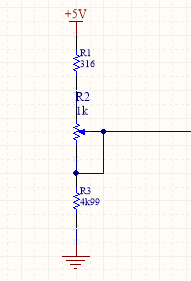
\includegraphics[scale=1]{Etapa-de-entrada.png}
	\caption{Etapa de entrada.}
	\label{fig:img_etapa-de-entrada}
\end{figure}

\noindent Para la implementación del comparador con histéresis se utiliza un amplificador operacional realimentado positivamente. Se implementa un ancho de histéresis de 26.665 mV,  alrededor de un punto de operación de 2.5 V, como se muestra en la figura \ref{fig:img_comp-con-hist}.

\begin{figure}[H]
	\centering
	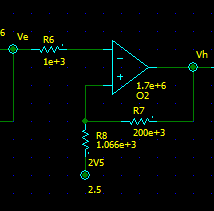
\includegraphics[scale=1]{Comparador-con-histeresis.png}
	\caption{Comparador con histéresis.}
	\label{fig:img_comp-con-hist}
\end{figure}

\noindent Para controlar la corriente en el electroimán se utiliza una topología en puente H, que permite conmutar la polaridad de la tensión aplicada a la bobina. Para medir la corriente se utiliza un sensor de efecto Hall, que es modelado en la simulación como  una fuente de tensión controlada por corriente, con una ganancia de 53.3 mV/A correspondiente a su transconductancia. Esta implementación puede observarse en la figura \ref{fig:img_puenteH}. Luego, su salida es realimentada a la etapa de entrada luego de restarle la tensión de referencia  $V_{bias}$ de 2.5V, como se muestra en la figura \ref{fig:img_resta-Vbias}. 

\begin{figure}[H]
	\centering
	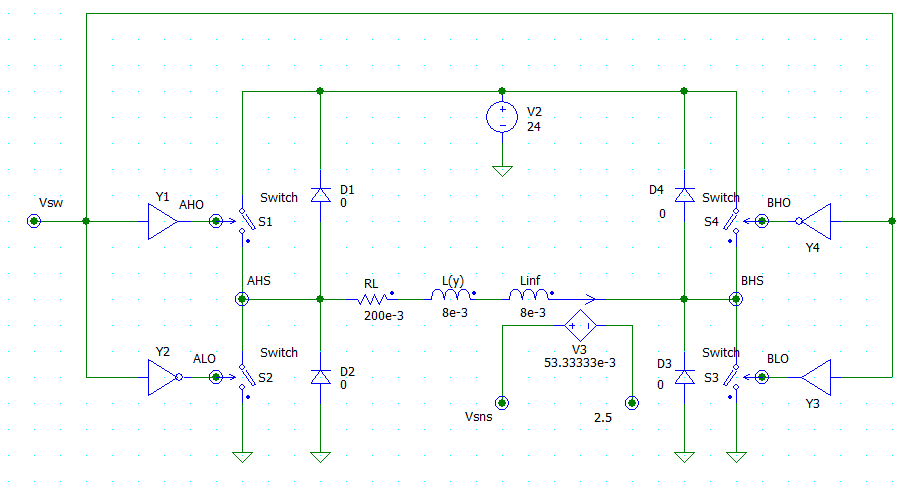
\includegraphics[scale=0.5]{PuenteH.png}
	\caption{Puente H y sensor de efecto Hall.}
	\label{fig:img_puenteH}
\end{figure}

\begin{figure}[H]
	\centering
	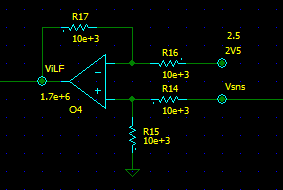
\includegraphics[scale=1]{Resta-Vbias.png}
	\caption{Resta del $V_{bias}$ al sensor de efecto Hall.}
	\label{fig:img_resta-Vbias}
\end{figure}

\subsubsection{Simulaciones de formas de onda}

\begin{figure}[H]
	\centering
	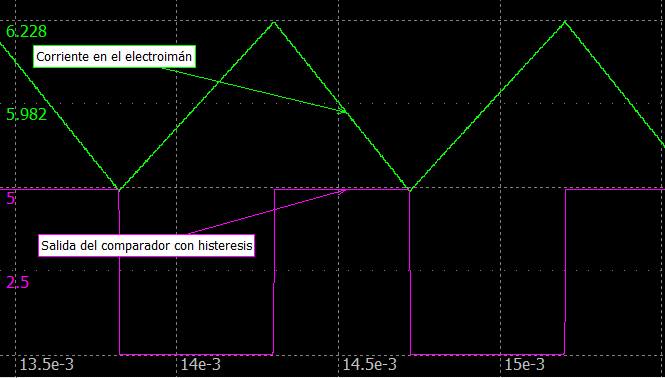
\includegraphics[scale=0.5]{Formas-de-onda-corriente.png}
	\caption{Formas de onda de corriente en el electroimán y salida del comparador.}
	\label{fig:img_formas-de-onda-corriente}
\end{figure}

\noindent En la figura \ref{fig:img_formas-de-onda-corriente} se pueden observar dos formas de onda. La inferior (violeta) se corresponde con la salida del comparador con histéresis, que conmuta. La onda triangular (verde) es la corriente en el electroimán. Para la simulación se utilizó una tensión de referencia de entrada de 1 V, por lo tanto el valor medio de la corriente en la salida es 6 A con un ripple de 500 mA. Esto fue verificado en la simulación mediante cursores.

\subsubsection{Simulación de un escalón en la referencia de corriente}

\noindent En la figura \ref{fig:img_respuesta-al-escalon} se muestra cómo cambia la corriente en el electroimán al aplicarle a la entrada del controlador un escalón de tensión entre 1 y 3 V. Se puede observar cómo la conmutación del comparador se detiene para ajustar la corriente con la referencia.

\begin{figure}[H]
	\centering
	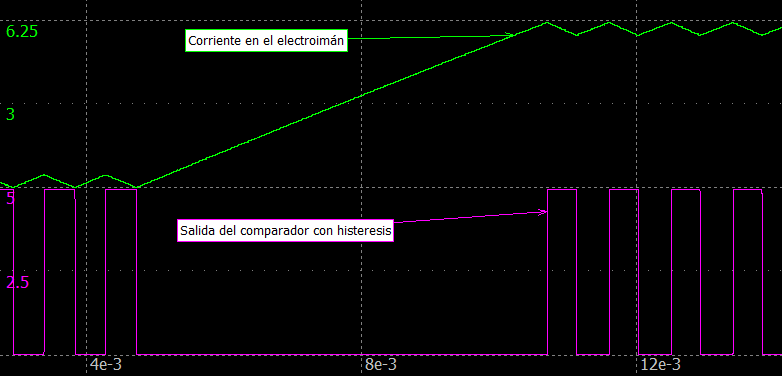
\includegraphics[scale=0.5]{Respuesta-al-escalon.png}
	\caption{Respuesta al escalón del circuito.}
	\label{fig:img_respuesta-al-escalon}
\end{figure}







